\documentclass[letterpaper, 10pt, journal]{IEEEtran}
\usepackage{graphicx}
\usepackage{float}
\usepackage{listings}
\usepackage{color}
\usepackage{multirow}
\usepackage[table,xcdraw]{xcolor}
\usepackage[justification=centering]{caption}
\usepackage[spanish]{babel}
\selectlanguage{spanish}
\usepackage[utf8]{inputenc}
% Paquete para referenciar figuras
\usepackage{nameref}
\graphicspath{ {./Images/} }
% Paquetes para las funciones matematicas
\usepackage{amsmath}
\usepackage{amssymb}

\usepackage[justification=centering]{caption}
\lstset{frame=tb,
  language=Java,
  aboveskip=3mm,
  belowskip=3mm,
  showstringspaces=false,
  columns=flexible,
  basicstyle={\small\ttfamily},
  numbers=none,
  numberstyle=\tiny\color{gray},
  keywordstyle=\color{blue},
  commentstyle=\color{dkgreen},
  stringstyle=\color{mauve},
  breaklines=true,
  breakatwhitespace=true,
  tabsize=3
}

\begin{document}
\title{Tarea 2 - 10 Experimentos Cient\'ificos Mas Bellos De La Historia }
\author{Kathy~Brenes~Guerrero, Barnum~Castillo~Barquero

~\IEEEmembership{
    \begin{center}
        Maestr\'ia en Ciencias de la Computaci\'on, Introducci\'on a la Investigaci\'on, ITCR
    \end{center}
}}% <-this % stops a space

% The paper headers
\markboth{Instituto Tecnol\'ogico de Costa Rica, Introducci\'on a la Investigaci\'on, Octubre~2018}%
{Shell \MakeLowercase{\textit{et al.}}: Tarea 2 - 10 Experimentos Cient\'ificos Mas Bellos De La Historia }
\maketitle

\begin{IEEEkeywords}

\end{IEEEkeywords}

\section{Introducci\'on}
El siguiente reporte detalla 10 experimentos considerados por nosotros como los mejores de algunas revistas de divulgacion cient\'ifica, que forman parte de los “10 experimentos cien\'ificos mas bellos de la historia”.

\section{Ca\'ida libre de los cuerpos realizado por Galileo en el siglo XVI}

\subsection{Historia de Galileo}

Galileo Galilei nació en Pisa el 15 de febrero de 1564, solo tres días antes de la muerte de Miguel Ángel, el último de los héroes del alto Renacimiento, a los 89 años de edad. Se cree que la familia de Galileo procedía del Mugello, un valle apartado a 24 kilómetros por caminos montañosos hacia el norte desde Florencia. Esta pequeña región aislada debió de contar con una despensa de genes notables, pues de allí salieron también los artistas Fra Angelico y Giotto, así como la familia Médicis. \cite{[1]}
\newline
El padre de Galileo, Vincenzo, procedía de una familia noble florentina que había conocido mejores tiempos. Tenía poco dinero y un carácter combativo que contribuía a mantenerle en esa situación. Pero era también un hombre de verdadero talento, había estudiado música en Venecia y se había convertido en un eminente experto en teoría musical. Se rebeló contra la camisa de fuerza del contrapunto, insistiendo en que la música debía agradar al oído en la práctica antes que a la mente en la teoría formal de la partitura. Sus composiciones influyeron en la liberación musical que desembocaría en el nacimiento de la ópera al final del siglo. \cite{[2]}
\newline
De tal palo, tal astilla. Galileo se convirtió en un mozo pelirrojo espabilado y presuntuoso cuya fachada encantadora y extrovertida ocultaba un temperamento algo más complejo. En casa, las cosas no eran fáciles. Su madre, Giulia, consideraba que se había casado por debajo de sus posibilidades. Con un inútil, decía ella. Esto no tardó en amargarla, convirtiéndola en una esposa regañona y una madre absorbente. Galileo se acostumbró a ser el centro de su atención, beneficiándose de la autoestima resultante, pero tras su carácter exuberante acechaban siempre las incertidumbres nacidas de su tormentosa vida familiar. \cite{[2]}
\newline
Cuando Galileo contaba diez años la familia se trasladó a Florencia, donde su padre se convirtió en músico de la corte y conocido polemista. Galileo fue enviado a educarse al monasterio de Vallombrosa, en los montes, a 24 kilómetros al este de la ciudad. 
\newline
En 1581, a los 17 años, Galileo volvió a su ciudad natal para estudiar medicina en la Universidad de Pisa. Su padre quería que se hiciera médico para que aportara unos muy necesarios ingresos a la familia.
\newline
Galileo adquirió la costumbre de colarse en las conferencias de Ricci, destinadas a los jóvenes de la corte. El intruso se armó de valor y se dirigió al maestro, haciéndole preguntas al acabar las conferencias. Ricci percibió enseguida su talento excepcional y le animó.
\newline
Galileo había encontrado por fin un maestro al que podía admirar. Ricci no era un matemático cortesano cualquiera. Era también un ingeniero militar excepcional. (Algunos años más tarde fue el encargado de reconstruir la fortaleza-islote del Château d’If frente a Marsella, cuyas fortificaciones describe Alejandro Dumas en su famosa novela, El Conde de Montecristo.) Ricci era la prueba de que se podía ganar dinero con las matemáticas si se destinaban a fines prácticos. \cite{[2]}
\newline
A Vincenzo no le hizo gracia enterarse de la escasa atención que su hijo dedicaba a sus estudios de medicina, pero ya empezaba a aceptar que este nunca sería médico: carecía del temperamento adecuado. Cuando la corte volvió a Florencia, Vincenzo abordó a Ricci y le preguntó si podría dar lecciones a Galileo. Ricci comenzó su instrucción con Euclides y Arquímedes. La claridad y el rigor de las argumentaciones de Euclides fueron una revelación para Galileo. Mientras que las argumentaciones escolásticas tradicionales apelaban a autoridades establecidas como la de Aristóteles, la autoridad para Euclides era la verdad, y solo esta se consideraba suficiente para probar sus proposiciones. En sus Elementos Euclides sentó las bases de la geometría y esbozó el método que habrían de adoptar los matemáticos. Comenzando por las definiciones más simples y evidentes en sí mismas (el punto, la línea) procedía luego a los teoremas, demostrando rigurosamente cada uno, que partía del anterior y así sucesivamente, construyendo de este modo el irrefutable edificio de la geometría.\cite{[1]}
\newline
Galileo no tardó en demostrar su talento excepcional en la esfera práctica. Como reza la historia muchas veces contada, un domingo, mientras escuchaba un largo sermón en la catedral de Pisa, se sintió intrigado por el balanceo de una lámpara sujeta al techo por medio de un largo alambre. Se percató de que la lámpara siempre tardaba el mismo tiempo en completar una oscilación, sin importar la amplitud del arco descrito en cada balanceo. En un arrebato de inspiración Galileo se dio cuenta de que se comportaba como el pulso. En cuanto llegó a casa construyó un péndulo con un hilo y una pesa de plomo. Realizó una serie de experimentos con diferentes pesos y diferentes longitudes de hilo. A partir de estos experimentos fabricó un aparato que podía usarse para tomar el pulso a un paciente. Lo mostró a algunos miembros del departamento de medicina de la universidad y quedaron tan impresionados que le robaron la idea de inmediato. Lo que obtuvo Galileo del pulsilogium, como vino a llamarse, fue un cierto renombre local. Cuando empezó a usarse en muchas otras ciudades italianas, Galileo no recibió dinero ni tampoco crédito por el invento. (El concepto de ley de patentes era todavía ajeno a la Italia del siglo XVI. El secreto, el plagio, el espionaje y la falsificación se consideraban parte del proceso de manufactura.)\cite{[2]}
\newline
Como resultado de esta práctica comercial, más otras a las que se entregaba Galileo en las tabernas, se le acabó el dinero. En 1685, después de cuatro años de universidad, volvió sin título a su casa de Florencia. Pero la falta de titulación no era suficiente para desanimar a alguien con tanta confianza en sí mismo. Se estableció enseguida como matemático, dando clases particulares cuando y donde podía. \cite{[1]}
\newline
La admiración de Galileo por los antiguos seguía intacta, pero no era nada propenso a la reverencia acrítica. Por esta época publicó una obra breve titulada La Balancietta.En ella describió el famoso experimento hidrostático realizado para determinar la cantidad de oro y plata empleadas en la manufactura de la corona de oro del rey Hierón (que según el fraudulento orfebre era de oro macizo). Después, Galileo tuvo la audacia de hacer mejoras sobre el experimento de Arquímedes, describiendo un método mucho mejor para determinar las proporciones de los distintos metales, empleando una balanza hidrostática de su propia invención. La balanza, conocida como balancietta, era un instrumento extremadamente delicado del mayor refinamiento técnico, capaz de detectar diferencias minúsculas de peso. Característico tanto de su época como de su inventor, era también un instrumento de gran belleza. Como su anterior pulsilogium, causó gran asombro a lo largo y ancho de Italia, pero una vez más la recompensa de Galileo fue una fama pasajera y no la fortuna. (Cada vez era más obvio su anhelo tanto de gloria como de riqueza.)\cite{[2]}
\newline
En muchos aspectos Galileo seguía siendo un hombre medieval. Su aceptación del pensamiento de la época, la autoridad de la iglesia e incluso de los cuentos de hadas literarios no se vio sacudida por su creciente conciencia científica. Su desprecio hacia la autoridad se restringía al único terreno en el que sabía lo que decía y sus oponentes no. En su mente coexistían lo medieval y lo moderno. De hecho, este conflicto entre dos mundos que no encajaban puede muy bien haber sido una fuente de estímulo. Shakespeare, contemporáneo de Galileo, tenía una mente similarmente dividida, y una actitud aún más esquizoide es manifiesta en su sucesor Newton, cuyo logro intelectual supremo fue mantener una firme creencia tanto en el mundo matemático de la astronomía como en el mundo mágico de la alquimia.\cite{[1]}
\newline
Había estudiado las obras de Arquímedes Del equilibrio de los planos y De conoides y esferoides. La primera era la obra seminal de la mecánica en la que Arquímedes formuló su «ley de la palanca»; en la segunda puso en práctica la ley que determina el centro de gravedad de una serie de paraboloides (el sólido formado al rotar una parábola sobre su eje). Genio y figura, Galileo se propuso aventajar a su héroe con el hallazgo de una manera práctica y original de descubrir el centro de gravedad de diversos esferoides. Galileo tardaría muchos años en publicar estos trabajos, pero circularon en forma manuscrita entre matemáticos de toda Italia, algunos de los cuales quedaron tan impresionados que tildaron a Galileo de «nuevo Arquímedes». Uno de ellos fue un marqués toscano llamado Guidobaldo del Monte, quien solo un año antes había publicado un extenso tratado de mecánica. Guidobaldo no era ningún diletante matemático (su tratado sería la obra fundamental sobre mecánica durante el siglo siguiente), y también estaba interesado en el centro de gravedad de los sólidos. Galileo fue a visitar a Guidobaldo y no tardaron en hacerse amigos. Compartieron sus hallazgos sobre la determinación de los centros de gravedad y Guidobaldo, muy impresionado, llamó la atención del nuevo gran duque de Toscana sobre la persona de Galileo.\cite{[2]}
\newline
El interés de los mecenas aristocráticos tiende a ser volátil, pero este no habría de ser el caso de Guidobaldo. Galileo había encontrado al fin un padrino constante y firme en su apoyo. Al quedar vacante el puesto de profesor de matemáticas en Pisa, Guidobaldo recomendó a Galileo de inmediato, y fue aceptado. Galileo reaccionó con júbilo. Al fin lo había conseguido. Solo después descubrió que su salario era de solo 60 coronas, más o menos lo que ganaba un tendero, y apenas suficiente para mantener a un hombre de las crecientes aspiraciones, apetitos y tamaño de Galileo. \cite{[2]}
\newline
La Universidad de Pisa no estaba preparada para el regreso de su díscolo hijo. El nuevo profesor de matemáticas (que no había logrado obtener un título en esta misma universidad) llegó con renovada confianza en sí mismo. Con sus 25 años, su abundante cabello rojo y su gusto por la controversia, se convirtió rápidamente en una figura popular, al menos entre los estudiantes.\cite{[2]}

\subsection{Experimento}
Galileo realizó su legendario experimento desde lo alto de la torre inclinada de Pisa, que confirmó su intuición previa acerca del granizo. Dejó caer dos objetos del mismo material y diferente peso, y cayeron a la misma velocidad. El más pesado no cayó a mayor velocidad, como debería haber hecho según Aristóteles.

El episodio es coherente no solo desde un punto de vista científico, sino también con la personalidad del protagonista, aunque la evidencia de que realmente tuviera lugar es tan nebulosa como la teoría que pretendía desacreditar. Aunque solo sea por su ejemplaridad merece consideración. Galileo quiso realizar una demostración pública de un error de Aristóteles, lo que ya es de por sí significativo dado que las enseñanzas de Aristóteles se consideraban como de una pieza, científicamente hablando. Cada elemento, cada ley, cada suposición se tenían por conexas entre sí. Al demostrar la falsedad de una de las partes, Galileo parecía sugerir la falsedad del todo, aunque no fuera esa su intención.

Como veremos, Galileo no pretendía tal osadía. A lo que se oponía en realidad era a la actitud aristotélica de fondo. La ciencia trata de los fenómenos de la realidad, y estos son mejor aprehendidos por la experiencia que por principios del pensamiento. Primero debía venir el experimento y, solo después, debía seguir la teoría. Llegados a este punto conviene señalar que Galileo nunca llegó a descubrir por qué los dos cuerpos caían a la misma velocidad. Esto no fue explicado hasta un siglo más tarde, cuando Newton formuló su ley de la gravedad: todo cuerpo en el universo atrae a otro a una fuerza que varía en proporción directa a sus respectivas masas y de modo inversamente proporcional al cuadrado de la distancia entre ellos. El mérito de Galileo es que recurrió a los resultados de la experiencia en lugar de a la teoría.

La trascendencia de lo que Galileo estaba haciendo era mucho más radical de lo que él estaba dispuesto a admitir, incluso para sus adentros, al menos en un comienzo. Pese a sus alardes públicos desde la torre inclinada, siguió dando lecciones sobre la física de Aristóteles. Esto no respondió a una actitud hipócrita ya que, en gran parte, parece haber creído en lo que enseñaba. Tomemos su visión del universo, por ejemplo. Copérnico había publicado ya en 1543, su propia teoría, en la que describía cómo los planetas giraban alrededor del Sol. Es seguro que Galileo sabía de esto, pero seguía creyendo en el modelo aristotélico establecido por Ptolomeo, con la Tierra firmemente colocada en el centro del universo y el Sol, la Luna y los planetas orbitando a su alrededor.

En este periodo Galileo creía en Arquímedes y Aristóteles. Podía ver que había discrepancias entre la postura esencialmente científica de Arquímedes y la esencialmente filosófica de Aristóteles, pero estaba seguro de que un día se podrían reconciliar. Fue también por estos años cuando Galileo escribió su primera obra relevante, Sobre el movimiento (De Motu). En su discurso a la Academia de Florencia sobre el infierno de Dante, había aplicado la ciencia a la literatura. Esta vez invirtió el proceso, pero con idéntica motivación. La combinación de las dos atraía a un público más amplio. Galileo era ambicioso y quería publicidad.

Habiendo prescindido de la noción aristotélica de que los cuerpos de diferente peso caen a diferente velocidad, Galileo proponía ahora una explicación diferente, basada en las conclusiones del experimento de la torre inclinada. Aquí Galileo puso en práctica lo que habría de ser su otro gran método científico: su habilidad para aprovechar las ideas de otros. En realidad, la explicación de Galileo de cómo cuerpos de diferente peso caen a la misma velocidad había sido propuesta casi 40 años antes por el físico veneciano Battista Benedetti (quien a su vez la «adaptó» a partir del principio de flotabilidad de Arquímedes). Galileo conocía sin duda el trabajo de Benedetti, su predecesor más ilustre en el campo de la física renacentista.

Benedetti tenía, como Galileo, una mentalidad dividida que nadaba entre dos aguas: las ideas medievales y las renacentistas. Era un científico de primera y un as de la astrología. Predijo su fallecimiento para el año 1592, pero se encontró en su lecho de muerte en 1590. Consiguió detectar un error en sus anteriores cálculos, lo cual le permitió morir con su fe zodiacal intacta. Ocasionalmente, también Galileo daría muestras de parecida alegría y desparpajo a la italiana a la hora de lidiar con las discrepancias.

Galileo estableció tres leyes del movimiento:
\begin{enumerate}
\item Todos los cuerpos caen de una misma altura en tiempos iguales.
\item Al caer los cuerpos, su velocidad total es proporcional al tiempo de caída.
\item El espacio recorrido por los cuerpos es proporcional al cuadrado de los tiempos.
\end{enumerate}
Galileo demostró estas leyes con sus experimentos sobre planos inclinados:

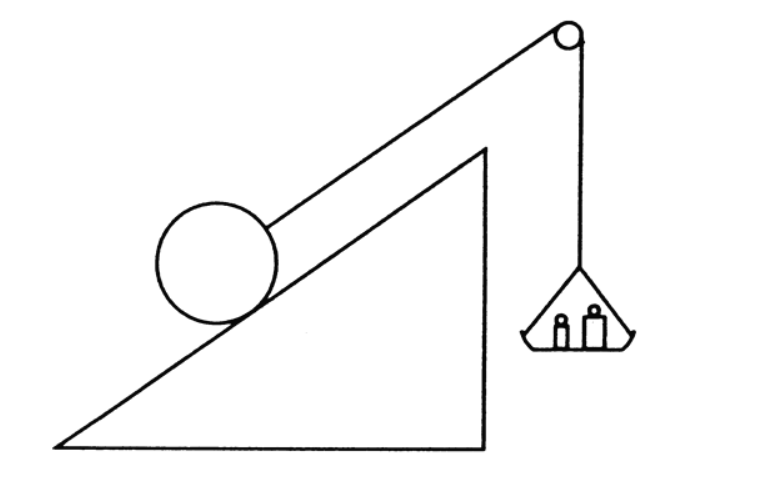
\includegraphics[scale=0.4]{Galileo1}

\subsection{Cronolog\'ia de la vida de Galileo}
\begin{description}
    \item 1564 - Nace en Pisa.
    \item 1581 - Comienza sus estudios de medicina en la Universidad de Pisa.
    \item 1585 - Se marcha de Pisa sin t\'itulo para vivir con su familia en Florencia.
    Empieza a dar clases.
    \item 1589  - Obtiene el puesto de profesor de matem\'aticas en la Universidad de Pisa.
    \item 1590  - Escribe De Motu.
    \item 1592 - Obtiene el prestigioso puesto de profesor de matemáticas en la Universidad de Padua.
    \item 1609 - El telescopio llega a Italia y es perfeccionado por Galileo.
    \item 1610 - Publica El nuncio sideral con gran éxito. Se traslada de Padua a Florencia bajo el mecenazgo del gran duque Cosme II.
    \item 1611 - Realiza una demostración de su nuevo telescopio en Roma.
    \item 1614 - Es atacado públicamente por la iglesia.
    \item 1616 - La iglesia le prohíbe «mantener o defender» el sistema copernicano.
    \item 1623 - Publica El ensayador. Maffeo Barberini se convierte en el papa Urbano VIII y permite a Galileo escribir un libro sobre las dos cosmologías rivales.
    \item 1632 - Tras ocho años de trabajo publica el Diálogo sobre los dos máximos sistemas del mundo. La iglesia le convoca a Roma.
    \item 1633 - El tribunal de la Inquisición le condena a cadena perpetua. Se retracta de su «ciencia herética».
    Vive bajo arresto domiciliario el resto de su vida.
    \item 1638 - El manuscrito de Discursos sobre dos nuevas ciencias es llevado clandestinamente a Holanda, donde se publica.
    \item 1639 - Se queda completamente ciego.
    \item 1642 - Muere a los 77 años.
\end{description}

\section{Experimento de la Gota de Aceite}
Robert Andrews Millikan es el responsable de llevar a cabo el Experimento de la Gota de Aceite. Robert Millikan es un físico experimental estadounidense (1868 - 1953) galardonado con el Premio Nobel de Física en 1923. 

Hijo del Reverendo Silas Franklin Millikan y Mary Jane Andrews y sus abuelos pertenecían a la población de Old New England, que había llegado a Estados Unidos antes de 1750, y eran colonos pioneros en el Medio Oeste. Dirigió una existencia rural en la infancia, asistiendo a la Maquoketa High School (Iowa). Después de trabajar por un corto tiempo como reportero de la corte, ingresó en Oberlin College (Ohio) en 1886. Durante su curso de licenciatura, sus asignaturas favoritas eran griego y matemáticas; pero después de graduarse en 1891 asumió durante dos años un puesto de profesor en física elemental. Fue durante este período que desarrolló su interés en el tema en el que más tarde iba a sobresalir.

Como científico, Millikan realizó numerosos descubrimientos trascendentales, principalmente en los campos de la electricidad, la óptica y la física molecular. Su primer gran éxito fue la determinación precisa de la carga transportada por un electrón, utilizando el elegante "Falling-drop method" (Experimento de la Gota de Aceite); también demostró que esta cantidad era una constante para todos los electrones (1910), demostrando así la estructura atómica de la electricidad. A continuación, verificó experimentalmente la importante ecuación fotoeléctrica de Einstein, y realizó la primera determinación fotoeléctrica directa de la constante h de Planck (1912-1915).

\subsection{Experimento}
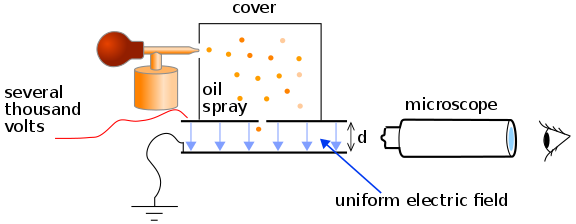
\includegraphics[scale=0.4]{dropmethod}
El experimento consistió en observar pequeñas gotas de aceite cargadas eléctricamente ubicadas entre dos superficies metálicas paralelas, formando las placas de un condensador. Las placas estaban orientadas horizontalmente, con una placa por encima de la otra. Se introdujo una neblina de gotas de aceite atomizado a través de un pequeño orificio en la placa superior y se ionizó mediante una radiografía, lo que las cargó negativamente.
 
Primero, con el campo eléctrico aplicado a cero, se midió la velocidad de una gota que caía. A la velocidad terminal la fuerza de arrastre es igual a la fuerza gravitacional. Como ambas fuerzas dependen del radio de diferentes maneras, el radio de la gota y, por lo tanto, la masa y la fuerza gravitacional podrían determinarse (utilizando la densidad conocida del petróleo). A continuación, se aplicó una tensión que induce un campo eléctrico entre las placas y se ajustó hasta que las gotas se suspendieron en equilibrio, lo que indica que la fuerza eléctrica y la fuerza gravitacional estaban en equilibrio. Usando el campo eléctrico conocido, Millikan podría determinar la carga en la gota de aceite. Al repetir el experimento con muchas gotas confirmaron que todas las cargas eran múltiplos enteros pequeños de un cierto valor base, que se encontró que eran $1.5924 (17) * 10^{-19}$ Coulomb, una diferencia de aproximadamente el 0,6\% del valor aceptado actualmente de $1.602176487 (40) * 10^{-19}$ Coulomb. Propusieron que esta era la magnitud de la carga negativa de un solo electrón.

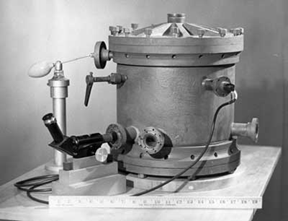
\includegraphics[scale=1.5]{dropmethod2}

\section{Experimento Perro de Parlov}
Ivan Petrovich Pavlov era un psicólogo ruso (1849-1936) mayormente conocido por su trabajo en el condicionamiento clásico. Su padre era Peter Dmitrievich Pavlov y era un sacerdote de aldea. Fue educado primero en la escuela de la iglesia en Ryazan y luego en el seminario teológico allí.

Inspirado por las ideas progresistas que D. I. Pisarev, el más eminente de los críticos literarios rusos de la década de 1860 y I. M. Sechenov, el padre de la fisiología rusa, Pavlov abandonó su carrera religiosa y decidió dedicar su vida a la ciencia. En 1870 se matriculó en la facultad de física y matemáticas para tomar el curso de ciencias naturales.

Pavlov se absorbió apasionadamente con la fisiología, que de hecho iba a seguir siendo de una importancia fundamental para él durante toda su vida. Fue durante este primer curso que produjo, en colaboración con otro estudiante, Afanasyev, su primer tratado aprendido, un trabajo sobre la fisiología de los nervios pancreáticos. Este trabajo fue ampliamente aclamado y fue galardonado con una medalla de oro por ello.

En 1890, Pavlov fue invitado a organizar y dirigir el Departamento de Fisiología del Instituto de Medicina Experimental (dirección que continuo por 45 años). Fue en el Instituto de Medicina Experimental en los años 1891-1900 que Pavlov realizó la mayor parte de su investigación sobre la fisiología de la digestión. 
La investigación de Pavlov sobre la fisiología de la digestión lo llevó lógicamente a crear una ciencia de los reflejos condicionados que daría forma el condicionamiento clásico. 

Junto con el condicionamiento operante, el condicionamiento clásico se convirtió en la base del conductismo, una escuela de psicología que dominó a mediados del siglo XX y sigue siendo una influencia importante en la práctica de la terapia psicológica y el estudio del comportamiento animal. El condicionamiento clásico es un proceso de aprendizaje básico, y sus sustratos neuronales están comenzando a entenderse.

\subsection{Experimento}

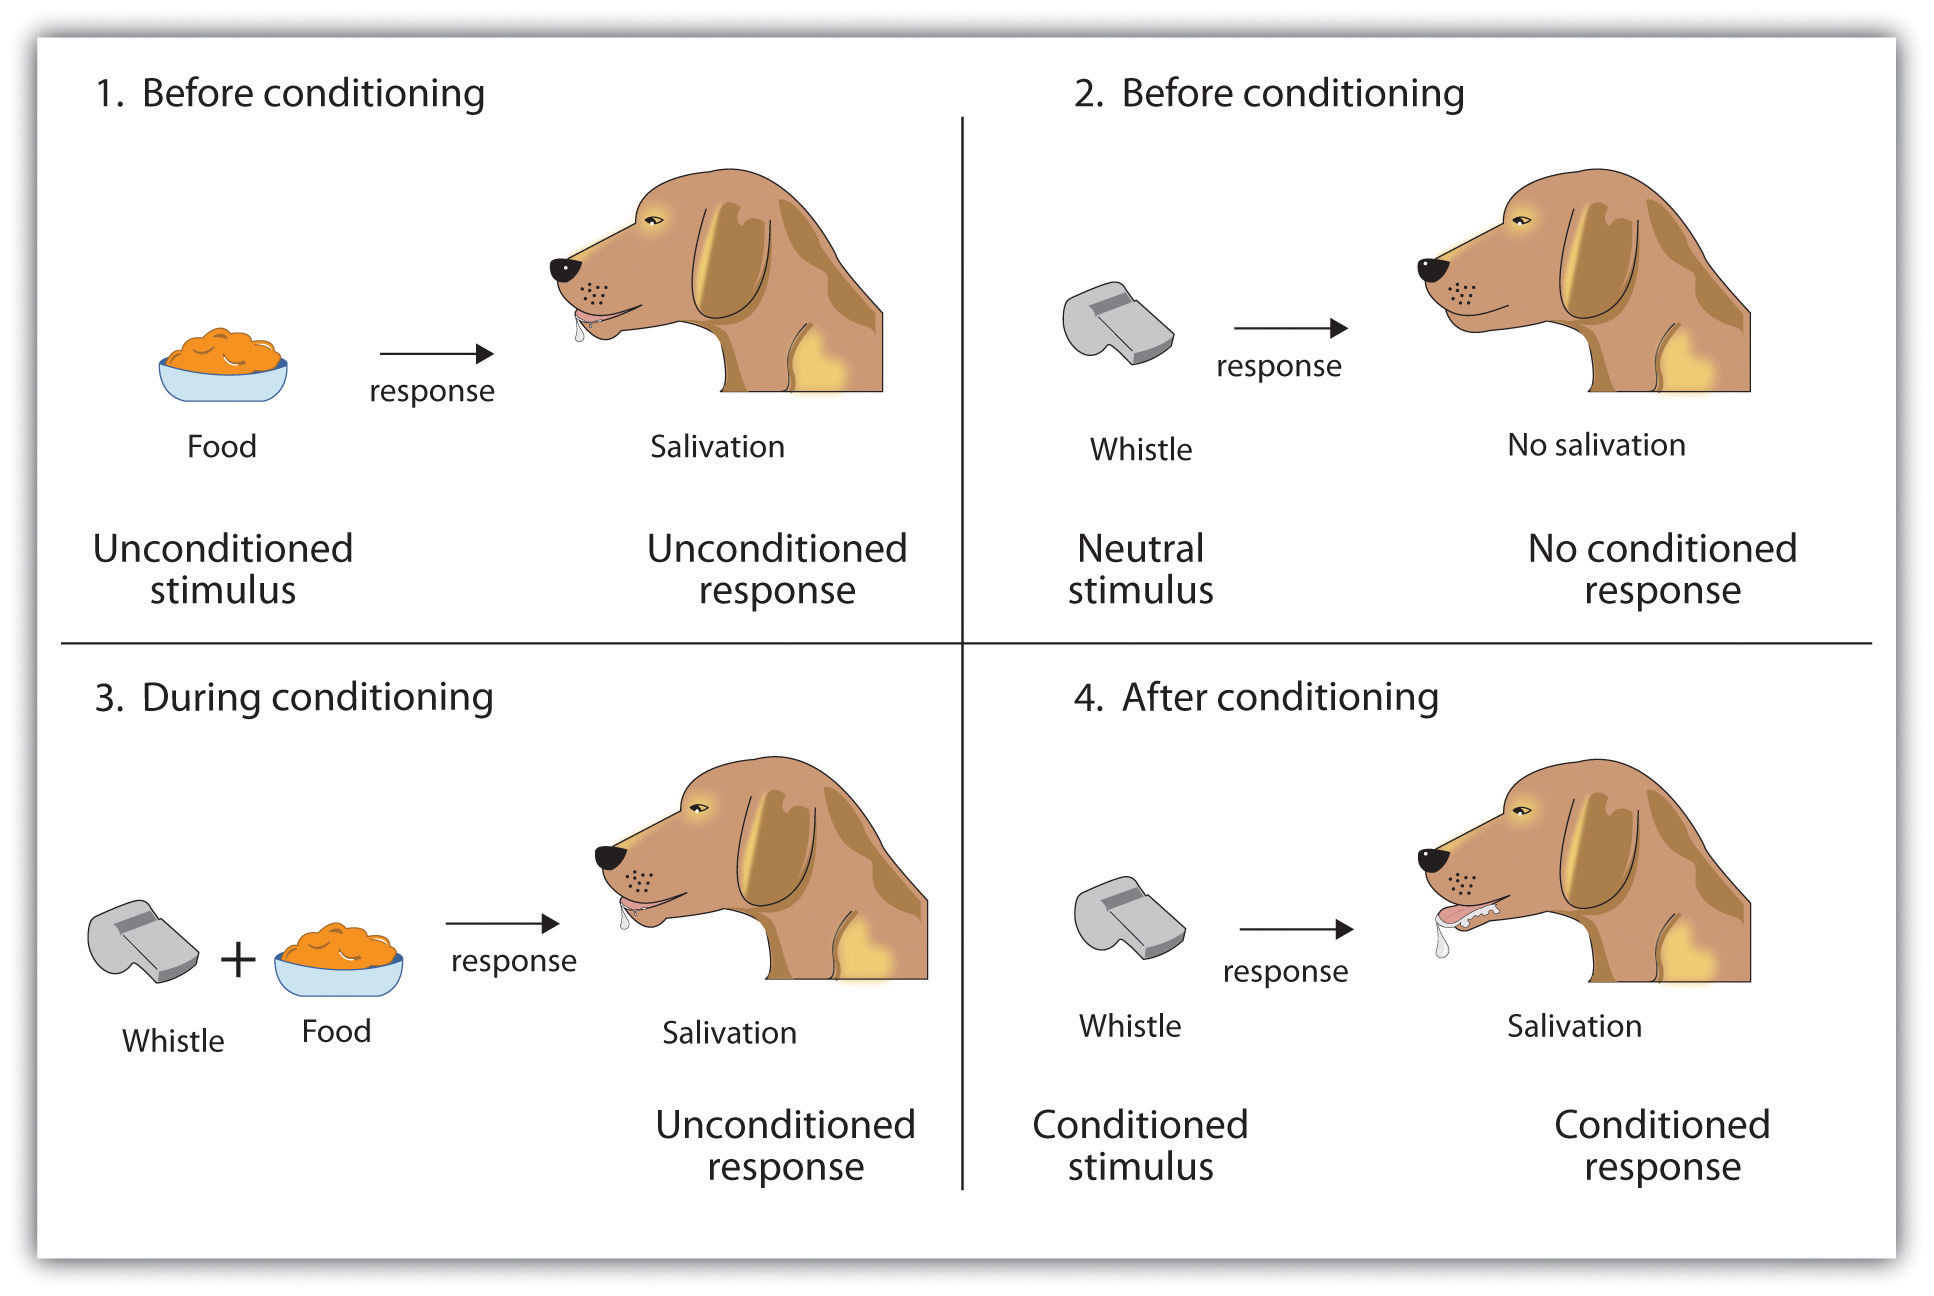
\includegraphics[scale=0.12]{parlov}

El experimento consiste en monitorear los reflejos de salivación en perros al presentarles alimento o un estímulo. El experimento se explica a continuación:

Los perros de Pavlov se colocaron en un entorno aislado y se sujetaron con un arnés, con un plato de comida frente a ellos y se usó un dispositivo para medir la velocidad a la que sus glándulas salivales formaban secreciones. Estas mediciones se registrarían en un tambor giratorio para que Pavlov pudiera monitorear las tasas de salivación a lo largo de los experimentos.

Encontró que los perros comenzaban a salivar cuando se abría una puerta para que el investigador los alimentara.

Esta respuesta demostró el principio básico del condicionamiento clásico. Un evento neutral, como abrir una puerta (un estímulo neutral, NS) podría asociarse con otro evento que siguió, en este caso, alimentado (conocido como el estímulo no condicionado, UCS). Esta asociación podría crearse repitiendo el estímulo neutral junto con el estímulo no condicionado, que se convertiría en un estímulo condicionado, lo que llevaría a una respuesta condicionada: la salivación.

Pavlov continuó su investigación y probó una variedad de otros estímulos neutrales que de otra manera no estarían vinculados a la recepción de alimentos. Estos incluían tonos precisos producidos por un zumbador, el tictac de un metrónomo, entre otras.

\section{Experimento Michelson-Morley}
Albert Abraham Michelson es el responsable de llevar el experimento a cabo junto con su asistente Edward Morley.

Michelson es un físico nacido en Prusia (1852 – 1931). Durante su carrera, Michelson se refirió a muchos departamentos de física, pero sobresalió en óptica. Realizó mediciones tempranas de la velocidad de la luz con asombrosa delicadeza y en 1881 inventó su interferómetro con el fin de descubrir el efecto del movimiento de la Tierra sobre la velocidad observada. En colaboración con el profesor E.W. Morley, y utilizando el interferómetro, se demostró que la luz viaja a una velocidad constante en todos los sistemas de referencia inerciales. El instrumento también permitió medir distancias con mayor precisión por medio de la longitud de las ondas luminosas. A solicitud del Comité Internacional de Pesos y Medidas, Michelson midió el medidor estándar en términos de longitud de onda de la luz de cadmio. 

Michelson ha contribuido numerosos artículos a muchas publicaciones científicas y entre sus trabajos más importantes están los clásicos, La velocidad de la luz (1902) Las ondas de luz y sus usos (1899-1903); y Estudios en Óptica (1927).

\subsection{Experimento}
La premisa del experimento era encontrar la presencia y las propiedades de una sustancia llamada éter, una sustancia que se cree llena el espacio vacío. 

Dado que las ondas en el agua necesitan algo para moverse (agua) y las ondas sonoras también (aire), se creía que la luz también necesitaba algo para moverse. Los científicos en el siglo XVIII llamaron a esta sustancia "éter", por el dios griego de luz. Creían que el éter estaba a nuestro alrededor y que también llenaba el vacío del espacio. El experimento lo hicieron con un dispositivo llamado interferómetro.

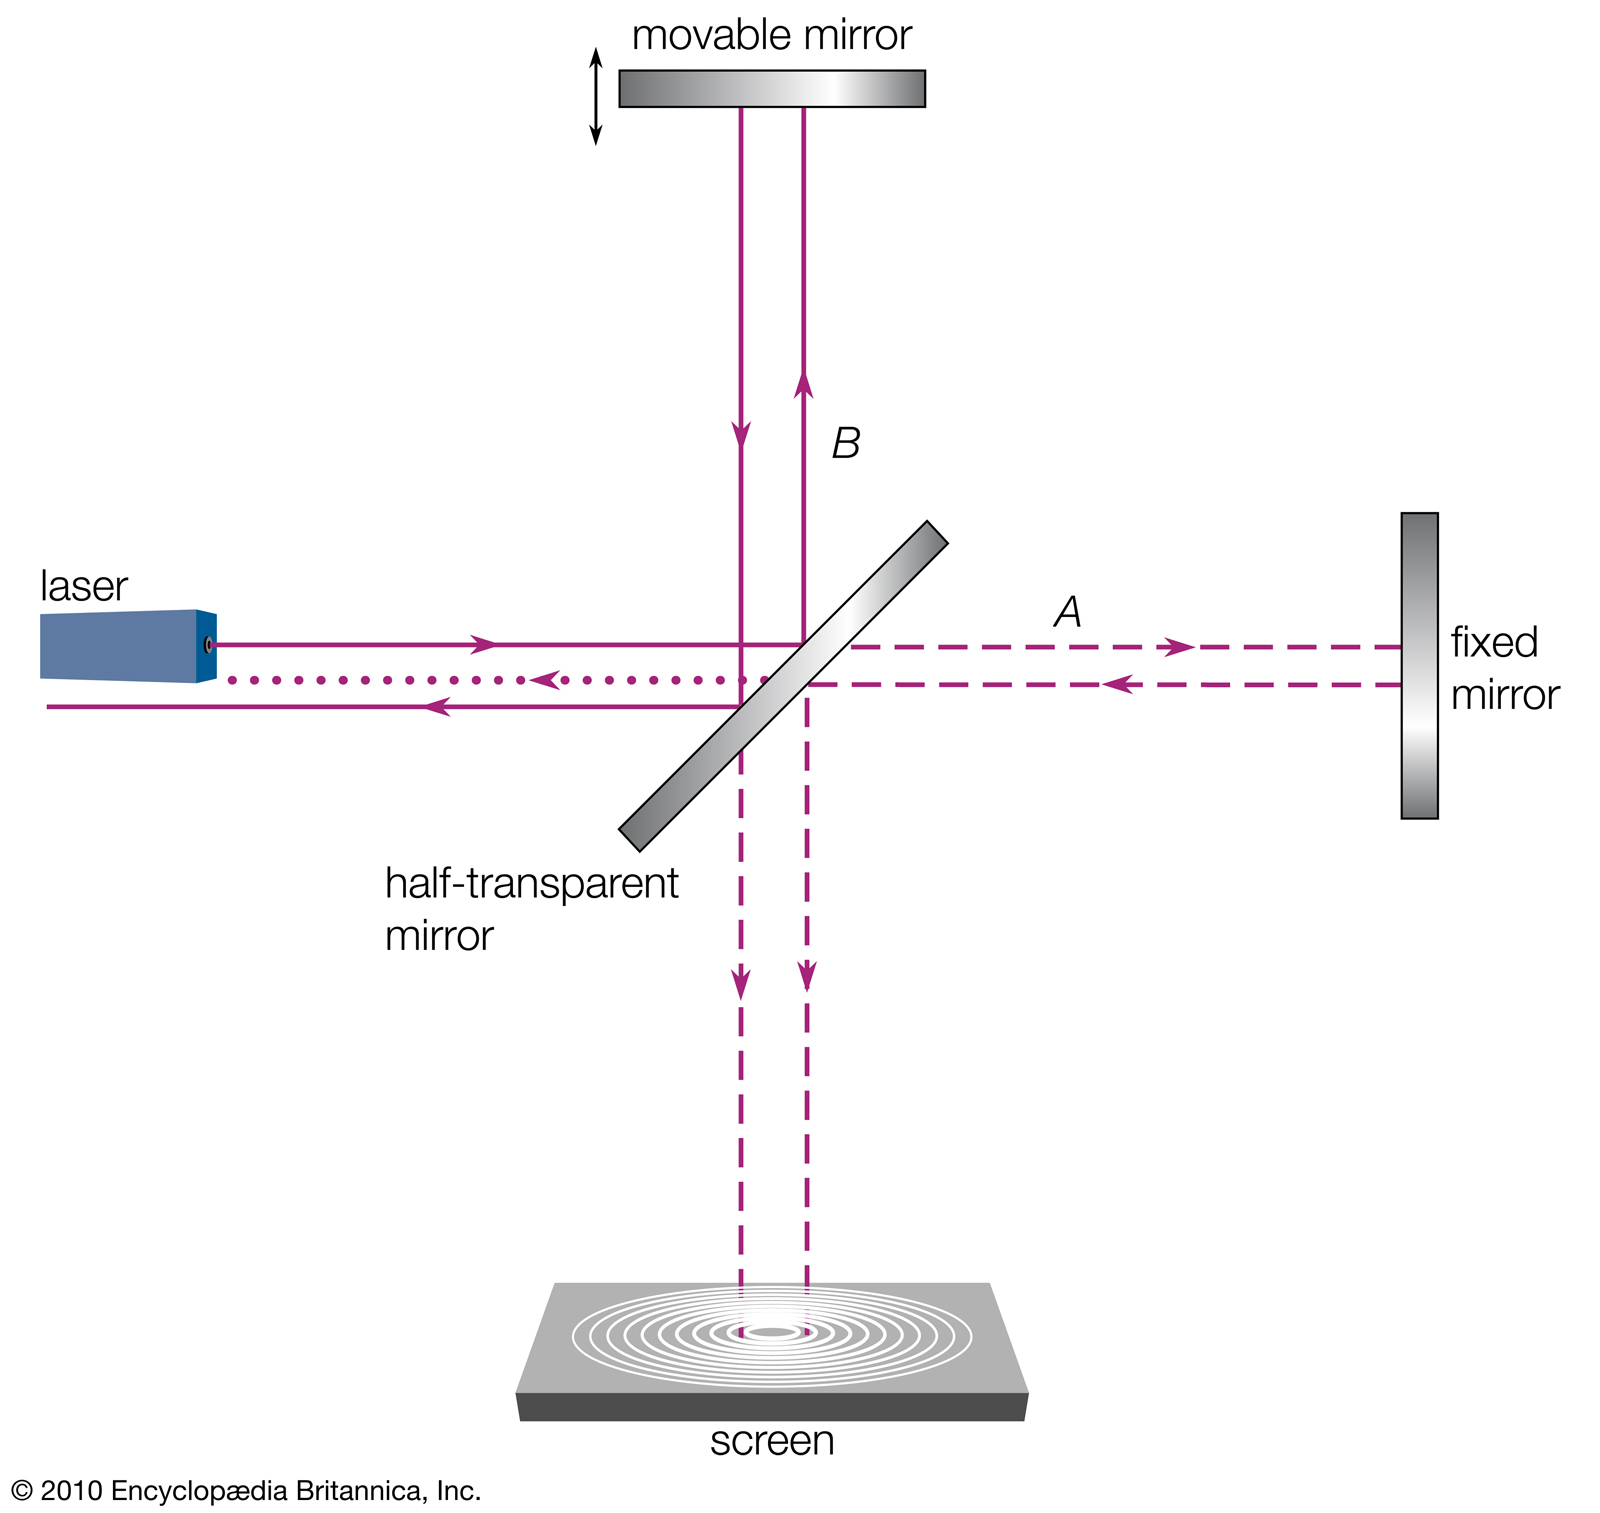
\includegraphics[scale=0.15]{luz}

La Tierra viaja rápidamente (más de 100.000 km por hora) alrededor del Sol. Si existe un éter, la Tierra que se mueve a través de ella causaría un "viento" de la misma manera que parece haber un viento fuera de un automóvil en movimiento. Para una persona en el automóvil, el aire fuera del automóvil parecería una sustancia en movimiento. De la misma manera, el éter debe parecer una sustancia en movimiento para las cosas en la Tierra.

El interferómetro fue diseñado para medir la velocidad y la dirección del "viento de éter" mediante la medición de la diferencia entre la velocidad de la luz que viaja en diferentes direcciones. Midió esta diferencia al hacer brillar un rayo de luz en un espejo que solo estaba parcialmente cubierto de plata. Parte de la viga se reflejaría de una manera, y el resto iría a la otra. Esas dos partes se reflejarán de nuevo en el lugar donde se dividieron y se combinaron. Al observar los patrones de interferencia en el haz de luz recombinada, se pueden ver los cambios en la velocidad debido al viento de éter.

Encontraron que no había una diferencia sustancial en las mediciones. Esto desconcertaba a la comunidad científica en ese momento y llevó a la creación de varias nuevas teorías para explicar el resultado. El más importante fue el factor de Lorentz que se usa en la teoría de la relatividad especial de Albert Einstein.

\section{Experimento de Phlogiston de Antoine Lavoisier}
Antoine-Laurent Lavoisier nació en una familia adinerada de la nobleza en París (1743- 1794). Hijo de un abogado en el Parlamento de París, heredó una gran fortuna a la edad de cinco años después de la muerte de su madre. Lavoisier comenzó su educación en el Collège des Quatre-Nations, Universidad de París (también conocido como Collège Mazarin) en París en 1754 a la edad de 11 años. En sus últimos dos años (1760–1761) en la escuela sus intereses científicos se despertaron y estudió química, botánica, astronomía y matemáticas.

Cuando Lavoisier, de 17 años, abandonó la Universidad de París en 1761, la química difícilmente podría considerarse una verdadera ciencia. A diferencia de la física, que había alcanzado la madurez a través del trabajo de Isaac Newton un siglo antes, la química todavía estaba atascada en el legado de los filósofos griegos. Los cuatro elementos de Aristóteles (tierra, aire, fuego y agua) fueron modificados lentamente por los alquimistas medievales, quienes agregaron su propio lenguaje y simbolismo arcanos.

Tirado en esta mezcla fue el concepto de phlogiston. Desarrollado por el científico alemán Georg Ernst Stahl a principios del siglo XVIII, phlogiston era un concepto químico dominante de la época porque parecía explicar mucho de una manera simple. Stahl creía que cada sustancia combustible contenía un componente universal de fuego, al que llamó phlogiston, de la palabra griega para inflamable. Debido a que una sustancia combustible, como el carbón, perdió peso cuando se quemó, Stahl razonó que este cambio se debía a la pérdida de su componente de phlogiston en el aire.

\subsection{Experimento}
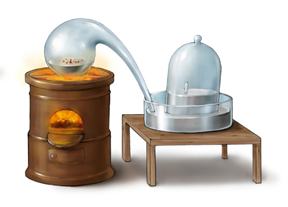
\includegraphics[scale=1.5]{caldera}

La imagen ilustra el experimento en el que Lavoisier quemó elementos de fósforo y azufre, demostrando que estos aumentaron de peso después de la combustión. Esto contradecía hipótesis del phlogiston, dado que cómo era posible que el phlogiston pesara menos que cero. Lavoisier le atribuyó el aumento del peso al aire que era absorbido durante la combustión.

Aunque Lavoisier ahora se dio cuenta de que la combustión realmente involucraba aire, la composición exacta del aire en ese momento no se entendía claramente. En agosto de 1774, el eminente filósofo natural inglés Joseph Priestley se reunió con Lavoisier en París. Describió cómo había calentado recientemente mercurio (un polvo rojo) y recogió un gas en el que una vela ardía vigorosamente. Priestley creía que su \textquotedblleft{}aire puro\textquotedblright{} mejoraba la respiración y hacía que las velas ardieran por más tiempo porque estaba libre de phlogiston. Por esta razón, llamó al gas que obtuvo de la descomposición de mercurio calx \textquotedblleft{}deflogisticated air\textquotedblright{}.

En París, el intrigado Lavoisier repitió el experimento de Priestley con mercurio y otros metales. Finalmente llegó a la conclusión de que el aire común no era una sustancia simple. En su lugar, argumentó, había dos componentes: uno que se combinaba con el metal y la respiración asistida y el otro un asfixiante que no soportaba ni la combustión ni la respiración. Para 1777, Lavoisier estaba listo para proponer una nueva teoría de la combustión que excluía el phlogiston. La combustión, dijo, fue la reacción de un metal o una sustancia orgánica con esa parte del aire común que calificó de \textquotedblleft{}eminentemente respirable\textquotedblright{}. Dos años más tarde, anunció a la Real Academia de Ciencias de París que descubrió que la mayoría de los ácidos contenían este aire respirable. Lavoisier lo llamó oxygène, de las dos palabras griegas para generador de ácido.

Lavoisier no esperaba que sus ideas fueran adoptadas de inmediato, porque aquellos que creían en el phlogiston \textquotedblleft{}adoptarían nuevas ideas sólo con dificultad\textquotedblright{}. Lavoisier puso su fe en la generación más joven que estaría más abierta a nuevos conceptos. Años después, en 1791, los resultados fueron evidentes. \textquotedblleft{}Todos los jóvenes químicos\textquotedblright{}, reflexionó, \textquotedblleft{}adoptan la teoría, y de ahí llego a la conclusión de que la revolución en la química ha llegado a suceder\textquotedblright{}. Su legado perdura más de 200 años después.

\section{Experimento de la Rueda de Paletas de James Joule}
James Joule fue un físico británico (1818 - 1889)  a quien se le debe la teoría mecánica del calor, y en cuyo honor la unidad de la energía en el sistema internacional recibe el nombre de Julio.

James Prescott Joule nació en el seno de una familia dedicada a la fabricación de cervezas. De carácter tímido y humilde, recibió clases particulares en su propio de hogar de física y matemáticas, siendo su profesor el químico británico John Dalton; compaginaba estas clases con su actividad profesional, trabajando junto a su padre en la destilería, la cual llegó a dirigir. Dalton le alentó hacia la investigación científica y realizó sus primeros experimentos en un laboratorio cercano a la fábrica de cervezas, formándose a la vez en la Universidad de Manchester.

A finales de la década de 1840, Joule se casó con Amelia Grimes y, no mucho después, los contemporáneos de Joule se volvieron más receptivos a su trabajo, en gran parte debido a su relación y colaboración con William Thomson (más tarde conocido como Lord Kelvin). Thomson, que había presenciado una de las conferencias de Joule a la Asociación Británica para el Avance de la Ciencia, estaba muy interesado en sus experimentos termodinámicos. Sin embargo, también estaba preocupado por su aparente conflicto con la entonces ampliamente aceptada teoría calórica propuesta originalmente por Antoine Lavoisier, que afirmaba que el calor existía como un tipo de fluido que fluía de cuerpos más cálidos a más fríos.

\subsection{Experimento}
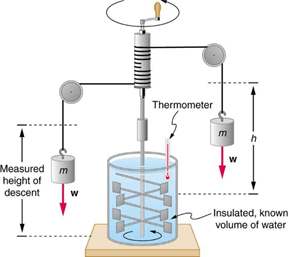
\includegraphics[scale=1.5]{paletas}

El experimento consiste en dos poleas con dos pesos en sus extremos, al caer el peso esta gira a través de un cilindro las paletas en un contenedor lleno de agua (1 lb).

El movimiento de la paleta calentó el agua y la relación fue precisa: elevar una libra de líquido en un grado llevó 772 libras-pie de trabajo. Joule había descubierto que el calor no era una cosa que fluía de un cuerpo a otro, sino una forma de movimiento.

\begin{thebibliography}{1}
\bibitem{[1]} Altshuler, J. (2002). \emph{A propósito de Galileo.} México: Secretaría de Educación Pública.
\bibitem{[2]} Strathern, P. (2017). \emph{Científicos en 90 minutos.} Pack 1. Madrid: Siglo XXI de España Editores, S.A. 

\bibitem{a} \emph{Latex-Tutorial.} (2018). Consultado desde https://www.latex-tutorial.com
\bibitem{b} \emph{ShareLatex.} (2018). Consultado desde https://www.sharelatex.com/learn
\bibitem{c} \emph{Sascha-Frank.} (2018). Consultado desde http://www.sascha-frank.com
\bibitem{[7]} \emph{Alineación de párrafos.} (2018). Consultado desde https://latextips.wordpress.com/2009/01/27/alineacion-de-parrafos/
\bibitem{30} \emph{Paddle wheel experiment} (2018). Consultado desde http://www.eoht.info/page/Paddle+wheel+experiment
\bibitem{31} \emph{James Prescott Joule} (2018). Consultado desde 
https://www.biografiasyvidas.com/biografia/j/joule.htm
\bibitem{32} \emph{Antoine Lavoisier 1743-1794} (2018). Consultado desde https://www.beautifulchemistry.net/lavoisier/
\bibitem{33} \emph{Albert Abraham Michelson Biographical} (2018). Consultado desde https://www.nobelprize.org/prizes/physics/1907/michelson/biographical/
\bibitem{34} \emph{Robert Andrews Millikan Biographical} (2018). Consultado desde https://www.nobelprize.org/prizes/physics/1923/millikan/biographical/
\bibitem{35} \emph{The Oil Drop Experiment: A Rational Reconstruction of the Millikan-Ehrenhaft Controversy and Its Implications for Chemistry Textbooks} (2000).
\end{thebibliography}
\end{document}






